\chapter{Frequency corrections for CO}
\label{chapter:freqCorrCO}

\smr\ measures \chem{CO} at an emission line resulting from the $J = 5 \rightarrow 4$ rotational transition, with a center frequency at 576.268 GHz. This is measured together with an \chem{O_3} line at a frequency band of 576.254 - 576.654 GHz in a stratospheric/mesospheric scan, corresponding to altitudes between roughly 7 km and 110 km. An example of such a measurement is shown in Figure \ref{fig:spectraCO}. 

\begin{figure}[ht!]
\begin{center}
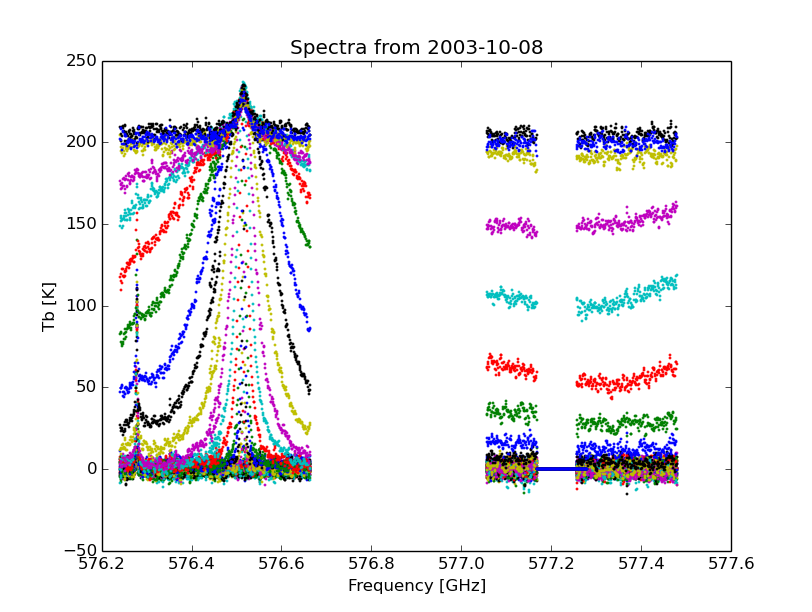
\includegraphics[width=0.7\textwidth]{freq_corr_coExample.png}
\caption{Brightness temperature spectra for altitudes ranging from 7 km to 110 km at the frequency band [576.254 - 576.654, 577.069 - 577.469] GHz (\smr\ frequency mode 22). The \chem{CO} line corresponds to the first peak at the lower frequency and the \chem{O_3} line measured simultaneously is shown at the higher frequency.}
\label{fig:spectraCO}
\end{center}
\end{figure}

The B1 frontend of \smr\ is used for all measurements of this \chem{CO} line, which sets the frequency range between 563 GHz and 581 GHz. The Phase-Lock Loop (PLL) in the \smr\ instrument (see Figure \ref{fig:blockdiagram}) controls the fine tuning of the frequencies to use for an observation, within the range set by the frontend. Due to a failure in the PLL component of B1, the local oscillator (LO) frequency is offset from the demanded frequency. For a year long period between 2003-10-08 and 2004-10-08, the PLL used for CO measurements was functioning, but all other observations were affected by this PPL malfunction. This has resulted in a frequency shift that varies from one scan to another in such a way that the lines can either be moved in a positive or negative direction, or lines might be missed completely in the observation. Examples of different shifts are shown in Figures \ref{fig:shiftExample1CO} and \ref{fig:shiftExample2CO}. In Figure \ref{fig:shiftExample2CO} it can be seen that there are measurements where \chem{CO} is not included in the spectra, which means that no data can be recovered.

\begin{figure}[ht!]
\begin{center}
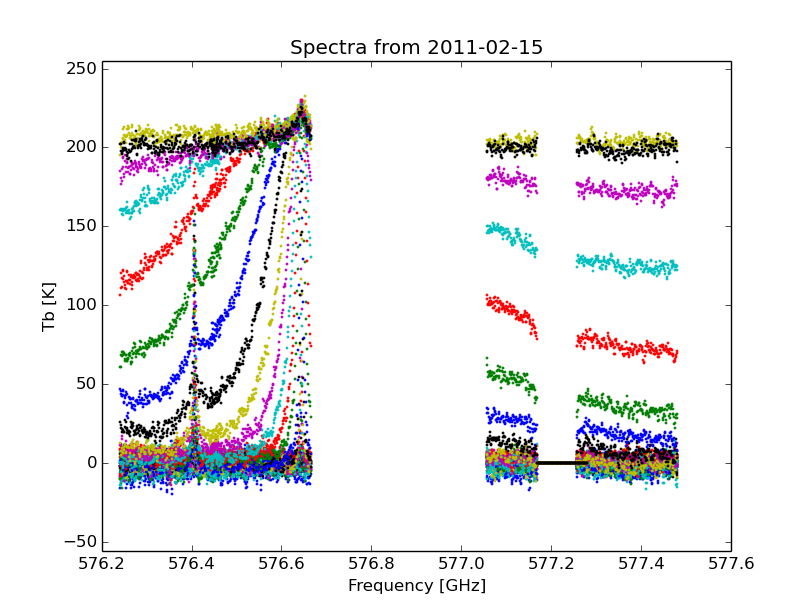
\includegraphics[width=0.7\textwidth]{freq_corr_errorSpectrum2.png}
\caption{Brightness temperature spectra measured 2011-02-15, showing an example of a frequency shift where both species are still included.}
\label{fig:shiftExample1CO}
\end{center}
\end{figure}

\begin{figure}[ht!]
\begin{center}
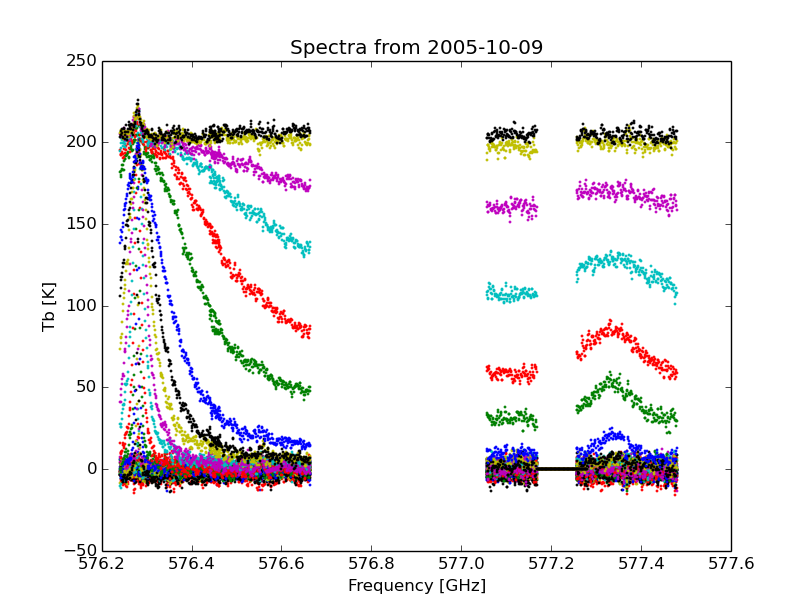
\includegraphics[width=0.7\textwidth]{freq_corr_errorSpectrum1.png}
\caption{Brightness temperature spectra measured 2005-10-09, showing an example of a frequency shift where only the \chem{O_3} line is included.}
\label{fig:shiftExample2CO}
\end{center}
\end{figure}

In order to correct the frequency shift, an algorithm has been developed and added to the retrieval process of \chem{CO}. Accurate frequency calibration is done in the algorithm by comparing the observed center frequency and the theoretical center frequency of 576.268 GHz of the \chem{CO} line, using the difference to shift the spectra. In order to do this, the \chem{CO} line must first be located by the algorithm and distinguished from the \chem{O_3} line. The distinction is performed by observing the slope of the brightness temperature measurements between altitudes of 40 km and 60 km, as is illustrated in Figure \ref{fig:altitudesCO}.

\begin{figure}[ht!]
\begin{center}
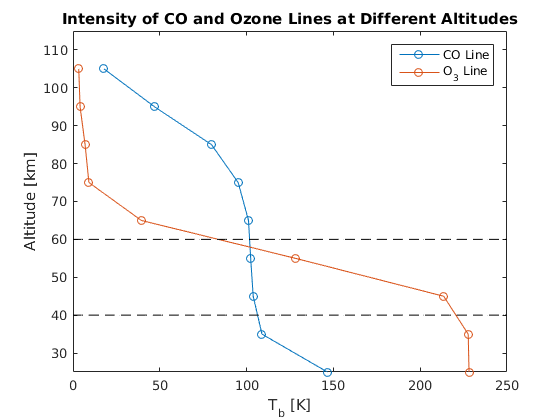
\includegraphics[width=0.7\textwidth]{freq_corr_altitudeProf.png}
\caption{Brightness temperatures, corresponding to the maximum of the peak of \chem{CO} and \chem{O_3}, at different altitudes. The values are averaged over observations between 2003-10-08 and 2004-10-08, when the PLL component was functioning. A clear difference between the red and blue curve can be observed in the slope between 40 km and 60 km.}
\label{fig:altitudesCO}
\end{center}
\end{figure}

A linear fit of the measured brightness temperatures with respect to altitude is performed between 40 km and 60 km. As can be observed in Figure \ref{fig:slopesCOO3}, there is a clear separation between the slopes of the different curves. If the obtained slope is larger than a cutoff chosen at -0.0045 K/m, the line is identified as \chem{CO} and the algorithm will continue to the next step of the correction. If no line is found in the measured spectra or if only the \chem{O_3} line is found, the scan is marked as unuseful and no additional corrections are made.

\begin{figure}[ht!]
\begin{center}
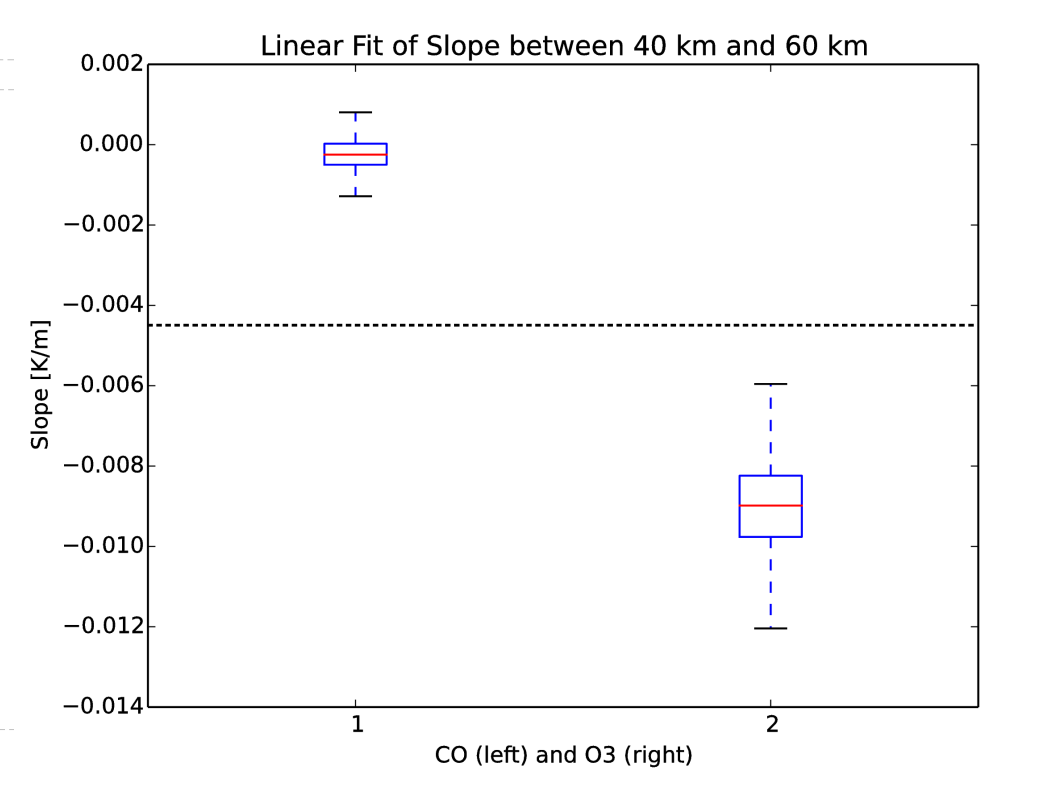
\includegraphics[width=0.7\textwidth]{freq_corr_slopeBox.png}
\caption{The slope of a linear fit of the brightness temperature between altitudes of 40 km and 60 km for \chem{CO} and \chem{O_3}. The data includes all observations between 2003-10-08 and 2004-10-08, when the PLL component was functioning. A cutoff between the two species can be observed around -0.0045 K/m.}
\label{fig:slopesCOO3}
\end{center}
\end{figure}

Once the observed \chem{CO} line has been located, the corresponding observed center frequency is determined. In order to do this, a Gaussian fit according to equation \eqref{equation:gaussFitCO} is applied to the measured data, where $b$ represents the center frequency. The difference between the obtained center frequency $b$ and the theoretical center frequency of 576.268 GHz is then applied to the local oscillator frequency of the radiometer, which means that all frequency values of the spectra are adjusted accordingly. The Gaussian fit and the correction are illustrated in Figure \ref{fig:gaussFitCO}.

\begin{equation}
    \label{equation:gaussFitCO}
    f(x) = a\cdot \exp \left (- \left (\frac{x-b}{c} \right )^2 \right )
\end{equation}

\begin{figure}[ht!]
\begin{center}
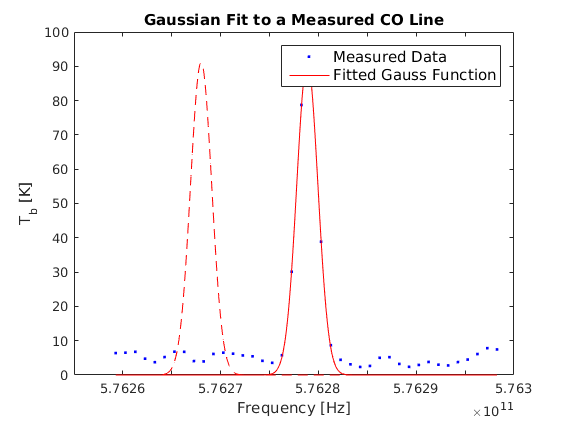
\includegraphics[width=0.7\textwidth]{freq_corr_gaussFit.png}
\caption{An example of measured brightness temperatures for \chem{CO} at a single altitude, together with a Gaussian fit of the values. The dashed red line shows the theoretical center frequency, where the line is shifted to.}
\label{fig:gaussFitCO}
\end{center}
\end{figure}

The amount of measurements that have been made, each year from 2001 until 2015, is shown in Figure \ref{fig:statisticsCO}, together with the number of measurements that could be recovered and the amount that could not. Table \ref{table:statisticsCO} shows the number of measurements that is affected and the number that is unaffected by the PLL malfunction, together with the precentage of the measurements that could be recovered in total and for each year between 2001 and 2015.

\begin{figure}[ht!]
\begin{center}
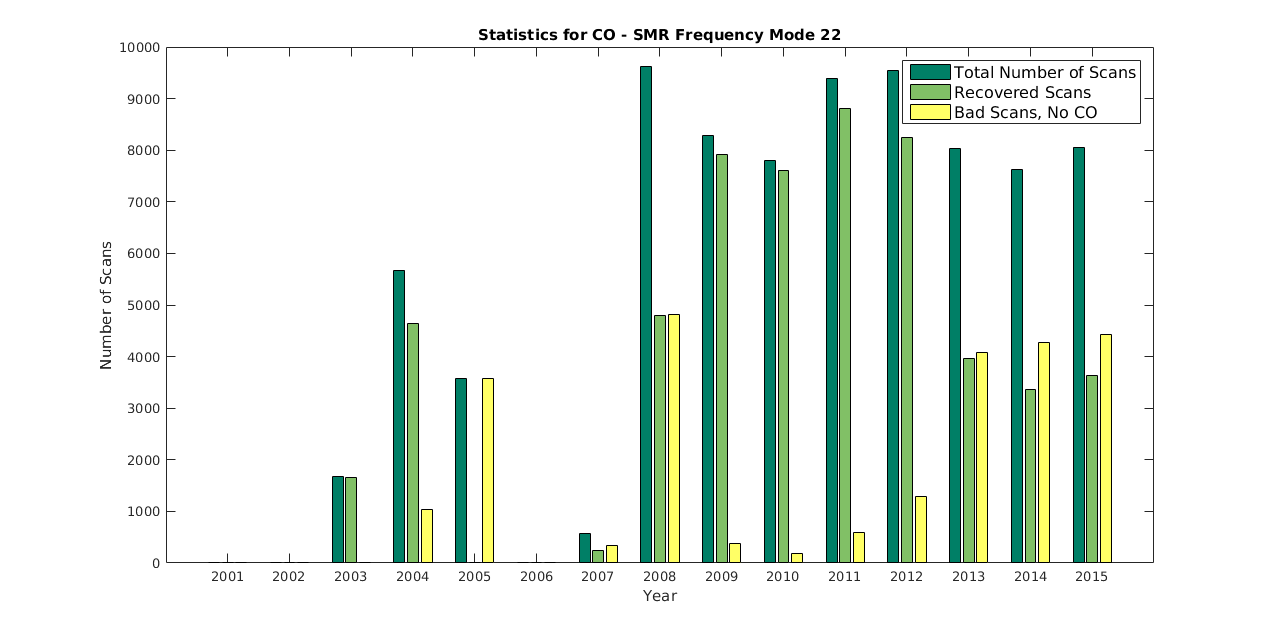
\includegraphics[width=0.9\textwidth]{freq_corr_statistics.png}
\caption{The amount of available data for \chem{CO} from frequency mode 22 of \smr\, calculated for each year ranging from the start in 2001 until 2015.}
\label{fig:statisticsCO}
\end{center}
\end{figure}


\begin{table}[ht!]
    \caption{The number of measurements that is affected and unaffected by the PLL malfunction, together with the precentage of the measurements that could be recovered. The data is displayed for each year from 2001 to 2015 and in total.}
    \label{table:statisticsCO}
    \begin{center}
        \begin{tabular}{|c|c|c|c|} \hline 
         \bf{Year} & \bf{\# Unaffected} & \bf{\# Affected} & \bf{Recovered [\%]} \\ \hline
         2001 & 0 & 0 & 0 \\ \hline
         2002 & 0 & 0 & 0 \\ \hline
         2003 & 1670 & 0 & 100 \\ \hline
         2004 & 4687 & 988 & 82 \\ \hline
         2005 & 0 & 3570 & 0 \\ \hline
         2006 & 0 & 0 & 0 \\ \hline
         2007 & 0 & 569 & 41 \\ \hline
         2008 & 0 & 9623 & 49 \\ \hline
         2009 & 0 & 8282 &  95 \\ \hline
         2010 & 0 & 7797 & 97 \\ \hline
         2011 & 0 & 9392 & 93 \\ \hline
         2012 & 0 & 9550 & 86 \\ \hline
         2013 & 0 & 8036 & 49 \\ \hline
         2014 & 0 & 7634 & 44 \\ \hline
         2015 & 0 & 8060 & 45 \\ \hline
         \bf{Total} & 6357 & 73501 & 68 \\ \hline
        \end{tabular}
    \end{center}
\end{table}

